\documentclass[11pt]{scrartcl}
\usepackage{outlines} 
\usepackage{enumitem}
\usepackage{multicol}
\setlength{\columnsep}{0.5cm}

\usepackage{amsmath,amssymb,amsthm}
\usepackage{geometry}

\geometry{letterpaper, margin=0.5in}
\usepackage{tikz}
\usetikzlibrary{automata,positioning,arrows,shapes.geometric}

\setlength\parindent{24pt}
\setenumerate[1]{label=\arabic*.}

\author{Jason Graalum}
\title{Asynchronous Implementation of a Bitonic Sorter}
\subtitle{CS 510 - Practicum in Asychronous System and Algorithms }
\date{}

\begin{document}
\maketitle

\section{Background}
\subsection{Bitonic Property}
A bitonic sorting algorithm makes used of the property that the array being sorted has only one change in "direction" or the array may be divided into two subarrays where one is monotonically increasing and the other is monotonically decreasing. We define a sequence having the "bitonic" property if:\\

$x_0 \leq ... \leq x_k \geq x\textsubscript{k+1} ... \geq x_n$ for some $k, 0 \leq k < n$\\

For an arbitrary stage of the bitonic sorter, the depth of comparators is log2 N where N is the number of words to compare.  Since this assumes that the words are in bitonic order, we need two previously sorted groups of words.  By reducing this down to the comparison of 2 words, we can find the total depth of the bitonic sorter:

$$Depth = \sum_{i=1}^{log_2N} i $$ where $N$ is the number of words being sorted. This means that each word is compared $Depth$ times. \\
Can can then determine the total number of comparators needed as:\\
$$\#\ of\ Comparators\ =\ (N\div2) \times \sum_{i=1}^{log_2N} i $$

\subsection{Bitonic Subsets}
Sorting algorithms are distinquished by how they decide which elements to compare and what to do based on the comparison.  For the Bitonic sorter, the monotonic property of the array of words allows the comparison of a selection of words which is built up from a simple comparison of two words to the comparison of two sets of $/n\/2$ words if sorting $n$ words.

For example, when sorting 8 words which may not have the bitonic property, we breakdown the problem by first comparing a subset of the array which is guaranteed to have the bitonic property - namely a 2-word subset. (Any two element subset, has the bitonic property.)
We then use the bitonic sorting algorithm to sort 2 words, then 4 words, then 8 words, etc.  We can use the bitonic algorithm in the manner because combining two previously sorted subsets of n words gives us a set of $n*2$ words that has the bitonic property.

\section{Asynchronous Justification}
The bitonic sorter relies on simple swaps of two data words. The latency in determining if the words are to be swapped or passed through is dependent on the bit differences of the word with a difference in the MSB resulting in a quick decision. Likewise, if the first bit difference is in the LSB, the latency is worst case(assuming we implement a quick "==" function.)
Due to this bit position variable latency, an asynchronous implementation of a parallel algorithm is well suited.

For this project, we will use the Full/Empty Asynchronous messaging as defined by (put reference to Roncken, et al.  Naturalized Communication and Testing -2015)

<need reference to Figure 4 from above paper?>\\

\section{Architecture}
\subsection{High Level System Architecture}
The bitonic sorter works by incrementally building bitonic lists starting with two words and doubling with each additional comparison level.  The example below shows a 8-word comparison network using 24 comparators. As shown above, the depth of the network is $\sum_{i=1}^{log_2N} i  = 1 + 2 + 3 = 6$. Assuming an average comparator delay of $D_{avg}$, the total delay is $D_{avg} * \sum_{i=1}^{log_2N} i$.


\begin{figure}[hbtp]
\centering
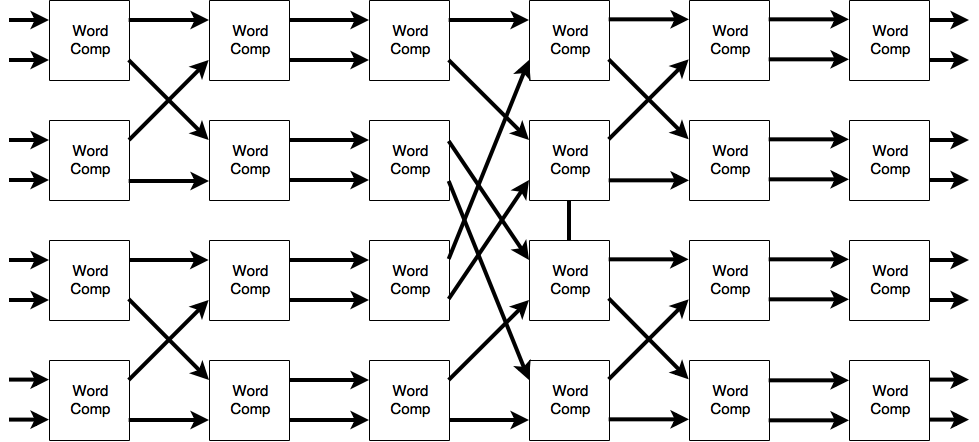
\includegraphics[scale=.40]{8_Word_Bitonic_Sorter_Diagram.png}
\caption{8 Word Bitonic Sorter}
\end{figure}

The interesting feature of an asynchronous implementation, is that the delay through the comparator is not fixed.  It depends on the data being compared - specifically the location of the first bit difference(starting at the MSB).

\begin{figure}[hbtp]
\centering
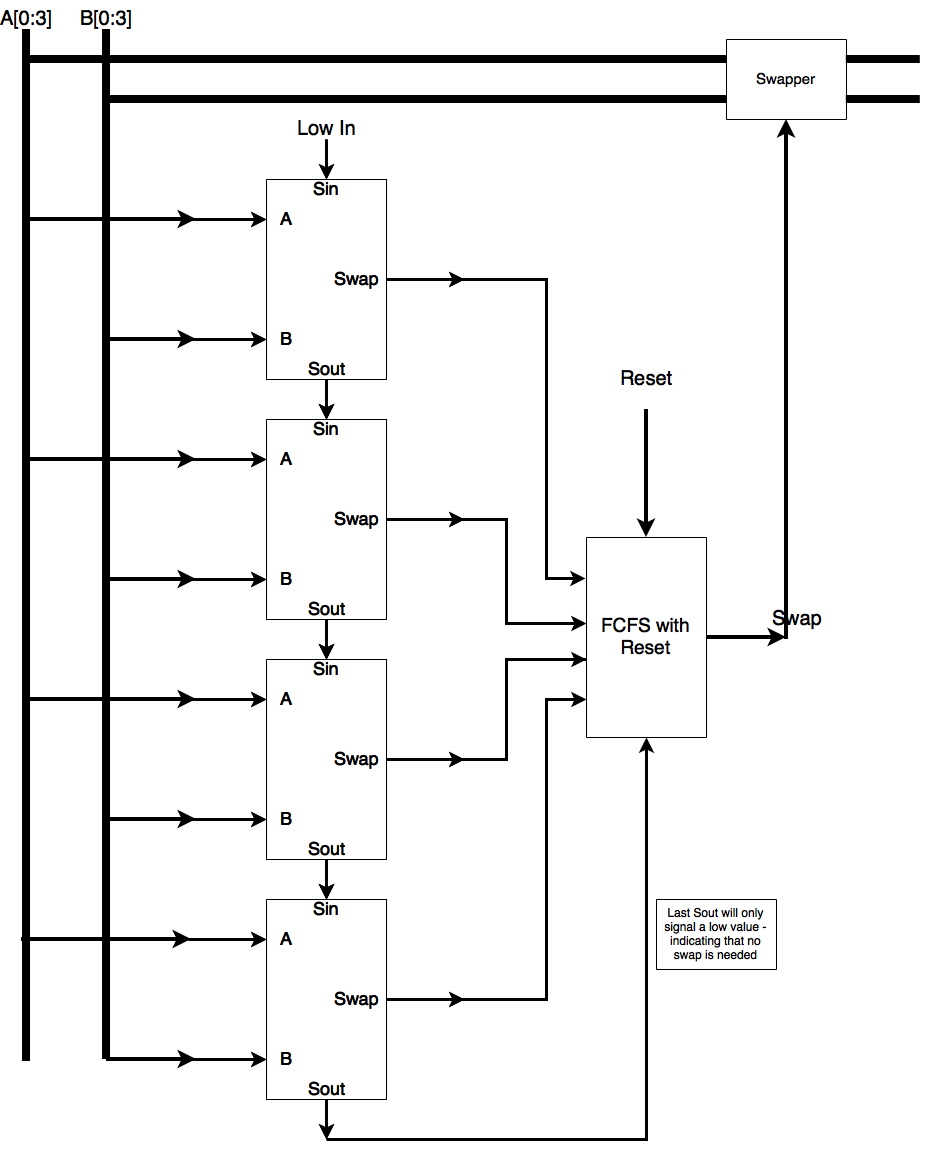
\includegraphics[scale=.40]{Word_Comparator_Block_Diagram.png}
\caption{4-Bit Word Comparator}
\end{figure}




\subsection{Word Comparator}
The word comparator takes as input two words under comparison. It outputs a single signal indicating whether the words should be swapped or simply passed through.
The word comparator breaks the comparison down by breaking out the two input words by bit. Each bit pair is routed to a single bit-comparator.  Starting at the MSB, the bit-comparator tests the inputs for a difference. If a difference is found, the comparator can make a decision requarding the ordering - and whether the Swap signal should be High or Low.  If a difference is not found, the MSB bit-comparator cannot make a decision. In this case, the Sout signal is asserted Low to tell the bit-comparator of the next bit that it needs to make a comparison. (In the case where a difference was found, the Sout signal is asserted Low telling the next comparator that a decision has been made.)\\  Similarly, if no difference is found, the comparisons continue down to the LSB.  At point, if no difference is found(i.e. the words are identical), the final Sout signal drives a low signal into the FCFS - this indicates that no swap is made. (Notice though that the level of the final Sout is High indicating a swap. But, as the words are identical, a swap is OK. This is done to eliminate the need to invert the final Sout signal.)

A key point here is that the comparison is NOT in parallel, but is sequential starting with the MSB. The best-case delay is if the MSB's are different. The delay in this case is 1  delay from A/B to Swap plus the FCFS delay.  The worst case is if the last bit is the same(or if there is no difference.) In this case, the delay is the word length times the delay from A/B to Sout plus the FCFS delay.


\subsection{Bit Comparator}


A and B are the unsorted input bits.  Sin is the "Swap Status" of the previous bit. (If the bit is the MSB, Sin is Low.)  A High value on Sin indicates that a swap decision has already been determined by previous higher-order bits.  If this is the case, the Swap output signal will NOT output any value. The Sin High value is also passed on to the next lower-order bit via the Sout signal.
A Low value on Sin indicates that no determination has been made by previous higher-order bits. In this case, A and B are compared. If they are different values, a value is driven onto Swap and Sout is pulled High. The A and B contain identical values, no value is drive on Swap and Sout is driven low - signalling the next comparator.\\

\begin{figure}[hbtp]
\centering
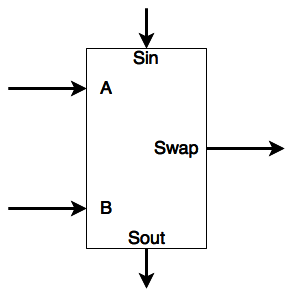
\includegraphics[scale=.8]{BitonicComparator_BlockDiagram.png}
\caption{Bitonic Comparator Block Diagram}
\end{figure}



\begin{table}
\centering
\begin{tabular}{ c | c | c || c | c  }
$Sin$ & $A$ & $B$ & $Sout$ & $Swap$  \\
\hline
0 & 0 & 0 & 0 & - \\
0 & 0 & 1 & 1 & 1 \\
0 & 1 & 0 & 1 & 0 \\
0 & 1 & 1 & 0 & - \\
1 & 0 & 0 & 1 & - \\
1 & 0 & 1 & 1 & - \\
1 & 1 & 0 & 1 & - \\
1 & 1 & 1 & 1 & - \\
\end{tabular}
\captionof{table}{Bitonic Comparator Truth Table} \label{tab:title} 
\end{table}

\subsection{FCFS - First-Come First-Server}


\section{Implementation}
\subsection{Circuit Implementation Considerations}
Given the bit-comparator truth tables\ref{bit comparator table} we can implement the function with simple logic gates.



\begin{figure}[hbtp]
\centering
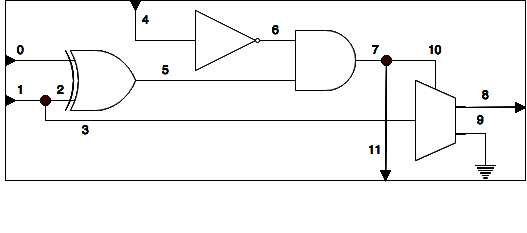
\includegraphics[scale=.7]{BitComparatorSchematic.png}
\caption{Bit Comparator Schematic}
\end{figure}


\subsubsection{Asynchronous}
\subsubsection{Latency}
Using a selection of random words, the chances that the MSB makes the decision is $50\%$. Likewise, each following bit has a $50\%$ chance to making the decision - i.e. it now becomes a comparison of n-1 bits. So, for a 4-bit word:

\begin{table}
\centering
\begin{tabular}{ c | c | c || c | c  }
Bit & Decision Chance & Cumulative Chance & Cumulative Delay   \\
\hline
3 - MSB & $50\%$ & $50\%$ & D + F \\
2           & $25\%$ & $75\%$ & 2D + F\\
1           & $12.5\%$ & $87.5\%$ & 3D + F\\
0 - LSB & $6.25\%$ & $93.75\%$ & 4D + F\\
ID & $2/2^n=6.25\%$ & $100\%$ & 4D + F\\


\end{tabular}
\captionof{table}{B4-Bit Word Comparison Distribution} \label{tab:title} 
\end{table}

So, the average delay is $(50\% \* (D + F) + 25\% \* (2D + F) + 12.5\% \* (3D + F) + 12.5\% \* (3D + F))/4$


\subsection{Physical Implementation}
\subsubsection{Single Bit Comparator}
\subsubsection{Word Comparator}
\subsubsection{Word-to-Word Proximity}

	      	   
\end{document}

